\subsection{Readspeaker}\label{readspeaker}
\emph{Readspeaker} maakt het mogelijk om webpagina's voor te lezen. Deze service is commercieel en kan via \url{http://www.readspeaker.com/} aangevraagd worden. 

Nadat je een geldig \emph{Readspeaker ID} hebt ontvangen kun je de functionaliteit activeren op de website. 

\textbf{Readspeaker activeren:}

\begin{enumerate}
\item Ga naar  \drupalpath{admin/config/dimpact/readspeaker}.
\item Selecteer bij \emph{Readspeaker status} de optie \emph{Activated}.
\item Vul bij het veld \emph{Readspeaker ID} je \emph{Readspeaker ID} in.
\item Klik op de knop \emph{Instellingen opslaan} om de instellingen op te slaan.
\end{enumerate}

\textbf{Readspeaker deactiveren:}

\begin{enumerate}
\item Ga naar  \drupalpath{admin/config/dimpact/readspeaker}.
\item Selecteer bij \emph{Readspeaker status} de optie \emph{Deactivated}.
\item Klik op de knop \emph{Instellingen opslaan} om de instellingen op te slaan.
\end{enumerate}

\begin{center}
	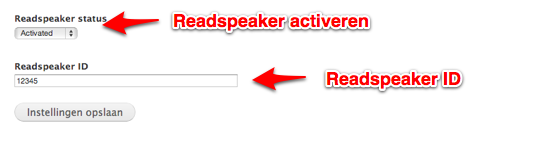
\includegraphics[width=\textwidth]{img/readspeaker.png}
\end{center}